\chapter{Marco Teórico}

\section{Automatización de pruebas}
La automatización de pruebas es una técnica usada en aplicaciones para
implementar todo el ciclo de vida del software en menor tiempo, y proveyendo a
este proceso de eficiencia y efectividad en su etapa de evaluación.

La automatización de las pruebas es mas útil en el lanzamiento de nuevas
versiones de software, para evaluar que todos los errores anteriormente
corregidos no sean introducidos nuevamente, mientras que será difícil y costoso
hacer las pruebas manualmente, ejecutar las pruebas automatizadas será mas
efectivo en términos de costo, uso de los recursos, y aprovechamiento del
tiempo.

Se conoce que en los siguientes escenarios es útil automatizar:

\begin{itemize}
    \item Los requerimientos no cambian frecuentemente.
    \item Se accede al aplicativo con múltiples y variados usuarios, roles y
        privilegios.
    \item El software es estable respecto a sus pruebas manuales.
    \item Se cuenta con el tiempo necesario para automatización en el proyecto.
    \item El proyecto sigue o debe seguir estándares estrictos.
    \item La complejidad del proyecto es elevada.
    \item El proyecto requiere constantes revisiones en algunas de sus
    características.
\end{itemize}

\subsection{Criterios a seguir}
Existen muchas herramientas útiles para escribir rutinas de automatización, pero
los pasos identificables en el proceso pueden simplificarse en los siguientes:

\begin{itemize}
    \item Identificar áreas dentro del software para automatizar.
    \item Elegir la herramienta adecuada para la automatización.
    \item Escribir las rutinas de prueba.
    \item Desarrollar el conjunto de casos de prueba.
    \item Ejecutar los casos de prueba.
    \item Generar los reportes de resultados.
    \item Encontrar los posibles errores o aspectos negativos.
\end{itemize}

\subsection{Beneficios}
Los beneficios de implementar un proceso de automatización de pruebas son
diversos, entre los cuales destacan:

\begin{itemize}
    \item Incremento de la productividad.
    \item Ahorro de dinero, en el costo del proyecto.
    \item Aumento de la calidad del software.
    \item Reducción del tiempo de evaluación del software.
    \item Soporte para múltiples aplicativos del software.
    \item Aumento de la cobertura de las pruebas.
    \item Reducción del trabajo repetitivo.
    \item Mejora de la consistencia del producto.
\end{itemize}

\subsection{Riesgos}
También existen riesgos implicados en la automatización de las pruebas, tales
escenarios deben ser considerados antes de proceder con la automatización, entre
estos están:

\begin{itemize}
    \item El costo de arranque de la automatización puede llegar a ser muy alto.
    \item Debe tenerse en cuenta que la automatización de las pruebas jamas
        podrá cubrir el 100\% de cobertura del software.
    \item No es conveniente automatizar una interfaz de usuario no establecida.
    \item Si la aplicación de usuario cambia constantemente, el costo de
        mantenimiento de las pruebas automatizadas será muy alto.
    \item Bajo ciertos paradigmas de implementación los testers podrían requerir
        tener un buen conocimiento de programación.
\end{itemize}

\section{Pirámide de la automatización de pruebas}
La pirámide de automatización de pruebas, es un concepto que fue introducido
por \emph{Cohn} en su articulo «\emph{Succeeding with Agile}», y describe como
equilibrar la automatización, comenzando con las pruebas unitarias en el nivel
mas bajo, y pasando a las pruebas de servicios; finalmente las pruebas de
interfaz de usuario se encuentran en la parte superior, como puede apreciarse en
la figura \ref{piramide}.

\begin{figure}
\centering
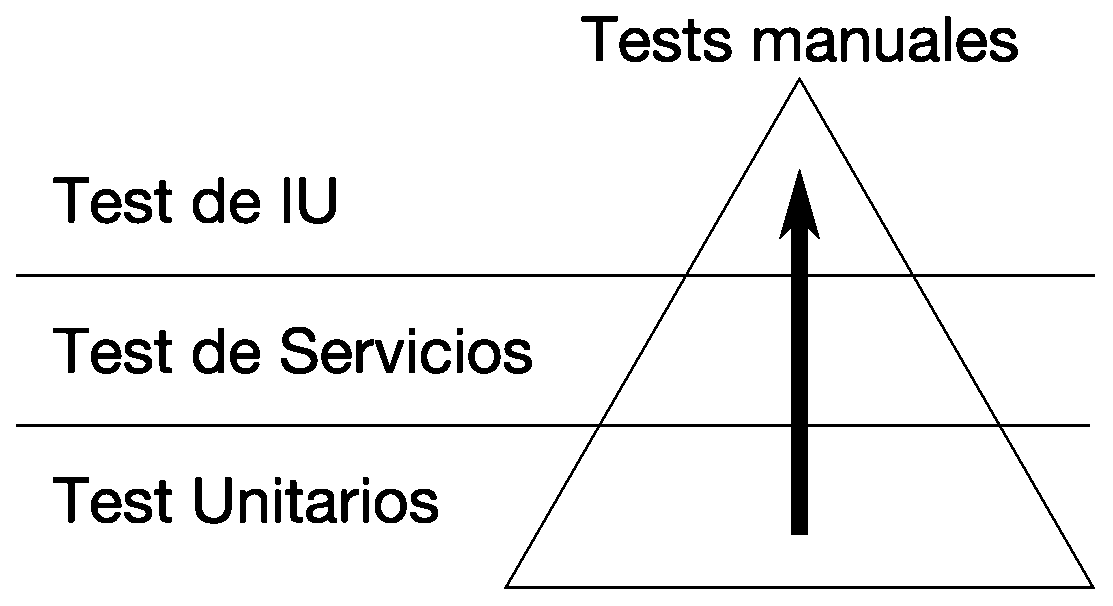
\includegraphics[width=0.5\textwidth]{graphics/pyramid.eps}
\caption{Pirámide de testing.}
\label{piramide}
\end{figure}

Las pruebas unitarias son rápidas y fiables, las pruebas en la capa de servicios
permiten evaluar la lógica del negocio donde la interfaz de usuario no esta
involucrada, cuanto mas alto sea el nivel en la pirámide, mas lentas y frágiles
resultan las pruebas.

Finalmente aunque se debe realizar alguna automatización de las pruebas de
interfaz de usuario, estas pruebas son mas lentas, mas difíciles de mantener y
se llegan a fallar mas fácilmente.

\subsection{La capa de interfaz}
Cuando el foco de la evaluación es la interfaz de usuario, se requiere que la
mayoría del código y la lógica de negocio este completamente evaluados. El
enfoque ahora se centra en simplemente asegurarse de que la propia interfaz de
usuario este funcionando correctamente. Las pruebas de interfaz de usuario son
muy frágiles, estas pruebas necesitaran mantenerse en cualquier momento que
cambie la interfaz de usuario, y como hay muchos factores que entran en juego
cuando se ejecuta una prueba que emula clics en una pantalla, estas pruebas
pueden dar como resultado falsos negativos. Estas fallas en las pruebas no
pueden ser ignoradas, pero tampoco debe gastarse mas tiempo en solucionar los
problemas y mantener las pruebas de UI que en encontrar defectos de código
reales.

Con un solido diseño de pruebas, las pruebas sobre la interfaz de usuario
complementan muy bien el conjunto de pruebas de automatización.

\section{End-to-End Testing}
Las pruebas End-to-End es una metodología que se utiliza para probar si el flujo
de una aplicación se esta realizando según lo diseñado de principio a fin. El
propósito de llevar a cabo pruebas de extremo a extremo es identificar las
dependencias del sistema y garantizar que la información correcta se transmita
entre varios componentes del sistema. Toda la aplicación se prueba en un
escenario del mundo real, como la comunicación con la base de datos, la red, el
hardware, y otros.

La prueba generalmente se realiza en la capa UI y se usa para validar que el
proceso de negocio de extremo a extremo funciona en todos los sistemas como una
prueba "horizontal". A diferencia de las pruebas verticales que miden el
rendimiento hacia arriba y hacia abajo de las capas de la pila de tecnología,
las pruebas horizontales de extremo a extremo se utilizan para garantizar que
los procesos de negocio de misión crítica funcionen. Las pruebas se ejecutan en
la capa UI y miden si la prueba continúa o no al siguiente paso del proceso.

\subsection{Buenas prácticas para pruebas E2E}
Una prueba típica de E2E puede ser compleja, con múltiples pasos que requieren
mucho tiempo para realizarlos manualmente. Esta complejidad también puede hacer
que las pruebas E2E sean difíciles de automatizar y lentas de ejecutar, para
ayudar a administrar los costos de las pruebas automatizadas de E2E a la vez que
mantienen los beneficios, se recomienda seguir las siguientes practicas:

\begin{itemize}
    \item Mantener una perspectiva de usuario final.
    \item Limitar las pruebas de excepción.
    \item Aplicar análisis de riesgo.
    \item Ejecutar las pruebas en el orden correcto.
    \item Manejar apropiadamente el entorno de prueba.
    \item Separar la lógica de prueba de los elementos de interfaz de usuario.
    \item Manejar correctamente la espera de los elementos de interfaz de usuario.
    \item Escoger los dispositivos adecuados.
    \item Optimizar el proceso de configuración y desmontaje de la prueba.
\end{itemize}

\section{Frameworks de automatización}
La automatización generalmente se interpreta como el manejo automático de
procesos a través de algoritmos inteligentes que involucran poca o ninguna
intervención humana. En el caso del software, significa realizar varias pruebas
en aplicaciones de software utilizando herramientas de automatización que son
versiones con licencia o de código abierto. En términos técnicos, el framework
de automatización de pruebas es un conjunto personalizado de componentes
interactivos que facilitan la ejecución de las pruebas con rutinas y la
generación de reportes completos de los resultados de las pruebas.

Dependiendo de como se desee abordar la creación de un framework y los
requisitos de automatización del proyecto, se cuentan con diferentes
clasificaciones:

\begin{description}
    \item [Lineal:] Son aquellos que registran los pasos de prueba y luego
        reproducir la rutina automáticamente para realizar la prueba.
    \item [Basado en módulos:] Estos dividen la aplicación bajo pruebas (AUT) en
        varios módulos lógicos y poco acoplados. Para cada modulo se crea una
        rutina de prueba separada e independiente.
    \item [De arquitectura de biblioteca:] Estos requieren determinar los pasos
        comunes de las pruebas, agruparlos en funciones en una biblioteca de
        funciones y llamar estas funciones en las rutinas de prueba cuando sea
        necesario.
    \item [Basado en datos:] Se enfoca en separar la lógica de las rutinas de
        prueba y los datos utilizados. Con esto se puede hacer que las rutinas
        de prueba funcionen fácilmente para diferentes conjuntos de datos.
    \item [Orientado por palabras clave:] Se enfoca en separar la parte técnica
        o de codificación del caso de prueba y de los pasos de necesarios de la
        prueba, para facilitar a una persona no técnica a entender bien la
        automatización.
    \item [Híbrido:] Son la combinación de dos o mas marcos mencionados
        anteriormente, que intenta aprovechar los puntos fuertes y los
        beneficios de otros marcos para el entorno de prueba.
\end{description}

